\chapter{Interacciones entre especies}\label{ch:b1:species-interactions}

En 1963, en una costa rocosa del Pacífico, un joven ecólogo empezó a
devolver al mar todas las estrellas de mar que encontraba en un tramo de
roca, y siguió haciéndolo durante años. Las estrellas de mar comían
mejillones. Sin ellas, los mejillones se extendieron roca abajo y desalojaron
a los percebes, las lapas, los quitones y las algas que habían vivido allí;
una \omterm{def:b1:ecosystem-organization:ecosystem}{comunidad} de quince especies cayó a ocho. Un solo depredador, ni
abundante ni grande, había estado manteniendo en su sitio a todo el
conjunto. Las especies no se limitan a compartir un lugar: compiten por él,
se comen unas a otras, viven dentro y encima unas de otras y dependen unas
de otras, y la \omterm{def:b1:ecosystem-organization:ecosystem}{comunidad} es la suma de esas interacciones. Este capítulo las
clasifica, da los modelos cuantitativos de \omterm{def:b1:species-interactions:types}{competencia} y \omterm{def:b1:species-interactions:types}{depredación} que un
primer año puede abordar, y muestra mediante experimentos cómo una sola
interacción puede modelar todo un \omterm{def:b1:ecosystem-organization:ecosystem}{ecosistema}.

\section{Una clasificación de las interacciones}

\begin{definition}[Interacciones interespecíficas]\label{def:b1:species-interactions:types}
\index{competencia}\index{depredación}\index{parasitismo}\index{mutualismo}\index{comensalismo}
Una interacción entre dos especies se clasifica por su efecto sobre cada
una: $+$ (beneficio), $-$ (perjuicio) o $0$. \emph{Competencia} ($-/-$):
ambas usan un recurso escaso. \emph{Depredación} ($+/-$): una mata y se come
a la otra; \emph{herbivoría} ($+/-$) cuando lo comido es una planta y suele
sobrevivir; \emph{parasitismo} ($+/-$) cuando el explotador vive sobre un
hospedador, o dentro de él, sin matarlo de golpe. \emph{Mutualismo}
($+/+$): ambas se benefician. \emph{Comensalismo} ($+/0$): una se beneficia
y la otra no se ve afectada. \emph{Amensalismo} ($-/0$): una sale
perjudicada y la otra no se ve afectada. Toda interacción es una presión
selectiva sobre los dos socios, y su adaptación recíproca a lo largo de las
generaciones es la \emph{coevolución}.
\end{definition}

\begin{example}[Un solo árbol, las seis]\label{ex:b1:species-interactions:oak}
Un roble compite con sus vecinos por la luz; los arrendajos se comen sus
bellotas (\omterm{def:b1:species-interactions:types}{depredación}) y las orugas, sus \omterm{def:b1:flowering-plant-organization:organs}{hojas} (herbivoría); el muérdago le
extrae la savia (\omterm{def:b1:species-interactions:types}{parasitismo}); sus raíces intercambian azúcares por fosfato
con un hongo (\omterm{def:b1:species-interactions:types}{mutualismo}); unos helechos crecen sobre su corteza y lo usan
solo como percha (\omterm{def:b1:species-interactions:types}{comensalismo}); y su sombra mata la hierba que hay debajo
(amensalismo).
\end{example}

\section{La competencia}

\begin{definition}[Competencia interespecífica]\label{def:b1:species-interactions:competition}
\index{exclusión competitiva}\index{reparto de nichos}\index{desplazamiento de caracteres}
Dos especies compiten cuando ambas usan un recurso --- alimento, luz, agua,
espacio, lugares de nidificación --- cuya disponibilidad limita su
crecimiento. La \omterm{def:b1:species-interactions:types}{competencia} puede ser por \emph{explotación} (cada una toma
lo que la otra habría usado) o por \emph{interferencia} (agresión directa,
toxinas, territorios). Su desenlace sigue el \emph{principio de exclusión
competitiva}: dos especies que necesitan el mismo recurso limitante de la
misma manera no pueden coexistir indefinidamente en un ambiente estable; la
mejor competidora elimina a la otra. Las competidoras que coexisten difieren
por tanto en \omterm{def:b1:ecosystem-organization:niche}{nicho} (\emph{reparto de \omterm{def:b1:ecosystem-organization:niche}{nichos}}) --- y allí donde dos especies
se solapan divergen a menudo en su forma más que donde cada una vive sola
(\emph{desplazamiento de caracteres}).
\end{definition}

\begin{proposition}[El modelo de competencia de Lotka--Volterra]\label{prop:b1:species-interactions:lotka}
Sean dos especies que crecen logísticamente (\cref{ch:b1:populations}) y sea
cada individuo de la especie 2 equivalente a $\alpha$ individuos de la
especie 1 en el uso del recurso de la especie 1, y cada uno de la especie 1
a $\beta$ de la especie 2:
\[
\frac{\dd N_1}{\dd t} = r_1 N_1\left(1 - \frac{N_1 + \alpha N_2}{K_1}\right),
\qquad
\frac{\dd N_2}{\dd t} = r_2 N_2\left(1 - \frac{N_2 + \beta N_1}{K_2}\right).
\]
La especie 1 deja de crecer sobre la recta $N_1 + \alpha N_2 = K_1$ (su
\emph{isoclina}\index{isoclina}), y la especie 2 sobre $N_2 + \beta N_1 = K_2$. Si
cada especie se limita a sí misma más de lo que limita a la otra ($\alpha <
K_1/K_2$ y $\beta < K_2/K_1$), las \omterm{prop:b1:species-interactions:lotka}{isoclinas} se cruzan con el equilibrio de
ambas especies estable y ambas \emph{coexisten}; si una \omterm{prop:b1:species-interactions:lotka}{isoclina} queda
enteramente por encima de la otra, esa especie \emph{excluye} siempre a la
otra; si cada una limita a la otra más que a sí misma, la ganadora depende
de los efectivos de partida.
\end{proposition}
\begin{proof}[Demostración parcial]
La especie 1 crece por debajo de su \omterm{prop:b1:species-interactions:lotka}{isoclina} y decae por encima; la especie
2, igual. Cuando las \omterm{prop:b1:species-interactions:lotka}{isoclinas} se cruzan con la de la especie 1 por encima
de la de la 2 en el eje $N_1$ y por debajo en el eje $N_2$, todo punto fuera
del cruce es empujado de vuelta hacia él desde cualquier lado: el cruce es
un equilibrio estable con ambas especies presentes. Cuando la \omterm{prop:b1:species-interactions:lotka}{isoclina} de la
especie 1 queda enteramente por fuera de la de la especie 2, todo punto
donde la especie 2 todavía podría crecer es también un punto donde la
especie 1 crece, y esta sigue creciendo después de que la 2 se haya
detenido, hasta alcanzar $K_1$ con $N_2 = 0$. El análisis completo se hace
en el volumen de segundo año; el esbozo de las \omterm{prop:b1:species-interactions:lotka}{isoclinas} da todos los
desenlaces sin él.
\end{proof}

\begin{omfigure}
\begin{tikzpicture}[font=\footnotesize, >=Stealth, line cap=round]
  \begin{scope}
    \draw[->, thick] (0,0) -- (4.6,0) node[below left] {$N_1$};
    \draw[->, thick] (0,0) -- (0,4.4) node[below right] {$N_2$};
    \draw[very thick, omDef] (4.0,0) -- (0,3.0) node[pos=0.15, above right, omDef!80!black] {la especie 1 se detiene};
    \draw[very thick, omThm] (2.6,0) -- (0,4.0) node[pos=0.85, right, omThm!80!black] {la especie 2 se detiene};
    \fill (1.63,1.78) circle (2pt); \node[anchor=west] at (1.75,1.95) {coexistencia estable};
    \draw[->, gray] (3.6,3.0) -- (2.2,2.2); \draw[->, gray] (0.4,0.4) -- (1.3,1.4);
    \node[anchor=north] at (2.3,-0.8) {cada especie se limita más a sí misma};
  \end{scope}
  \begin{scope}[xshift=7.2cm]
    \draw[->, thick] (0,0) -- (4.6,0) node[below left] {$N_1$};
    \draw[->, thick] (0,0) -- (0,4.4) node[below right] {$N_2$};
    \draw[very thick, omDef] (4.0,0) -- (0,4.0) node[pos=0.5, above right, omDef!80!black] {la especie 1 se detiene};
    \draw[very thick, omThm] (2.4,0) -- (0,2.4) node[pos=0.35, anchor=north east, align=right, omThm!80!black] {la especie 2\\ se detiene};
    \fill (4.0,0) circle (2pt); \node[anchor=north, font=\scriptsize] at (3.5,-0.3) {la especie 1 sola en $K_1$};
    \draw[->, gray] (1.0,3.4) -- (2.1,2.3); \draw[->, gray] (2.4,2.0) -- (3.4,0.7);
    \node[anchor=north] at (2.3,-0.8) {la especie 1 gana en todas partes};
  \end{scope}
\end{tikzpicture}

{\small Dos desenlaces de la \omterm{def:b1:species-interactions:types}{competencia} entre dos especies, leídos en las
\omterm{prop:b1:species-interactions:lotka}{isoclinas} (las rectas donde cada especie deja de crecer). Izquierda: las
\omterm{prop:b1:species-interactions:lotka}{isoclinas} se cruzan de modo que a cada especie la frena más ella misma que
la otra, y coexisten. Derecha: la \omterm{prop:b1:species-interactions:lotka}{isoclina} de la especie 1 queda por fuera
de la de la especie 2, y la especie 1 gana siempre.}
\end{omfigure}

\begin{proposition}[Exclusión competitiva]\label{prop:b1:species-interactions:gause}
\index{principio de Gause}
Dos especies que compiten por un único recurso limitante en un ambiente
constante no pueden persistir ambas: aquella cuya \omterm{def:b1:populations:population}{población} puede seguir
creciendo con el recurso a un nivel más bajo lo lleva por debajo de lo que
la otra necesita, y la otra decae hasta extinguirse.
\end{proposition}
\begin{proof}[Evidencia]
Gause (1934) cultivó dos ciliados, \emph{Paramecium aurelia} y
\emph{P.~caudatum}, con una ración diaria de bacterias. Por separado, cada
uno creció logísticamente hasta su propia meseta. Juntos, \emph{P.~aurelia},
que crece más deprisa y necesita menos alimento por individuo, alcanzó casi
su meseta mientras que \emph{P.~caudatum} decayó hasta desaparecer en
dieciséis días. Una tercera especie, \emph{P.~bursaria}, que se alimenta en
el fondo del tubo, donde \emph{P.~aurelia} no lo hace, coexistió con ella
indefinidamente: la exclusión se cumplía solo cuando los \omterm{def:b1:ecosystem-organization:niche}{nichos} eran iguales.
\end{proof}

\begin{omfigure}
\begin{tikzpicture}
\begin{axis}[
  width=0.8\linewidth, height=6.2cm,
  axis x line=bottom, axis y line=left,
  xmin=0, xmax=20, ymin=0, ymax=220,
  xlabel={días}, ylabel={individuos por \qty{0.5}{mL}},
  xlabel style={font=\small}, ylabel style={font=\small},
  tick label style={font=\small},
  legend style={font=\scriptsize, at={(0.98,0.02)}, anchor=south east, draw=none, fill=none},
  legend cell align=left,
]
\addplot[omDef, very thick, dashed, domain=0:20, samples=60] {200/(1+40*exp(-0.8*x))};
\addlegendentry{\emph{P.~aurelia} sola}
\addplot[omThm, very thick, dashed, domain=0:20, samples=60] {130/(1+25*exp(-0.55*x))};
\addlegendentry{\emph{P.~caudatum} sola}
\addplot[omDef, very thick, domain=0:20, samples=60] {170/(1+40*exp(-0.65*x))};
\addlegendentry{\emph{P.~aurelia} en mezcla}
\addplot[omThm, very thick, domain=0:20, samples=80] {80*exp(-0.05*(x-6)^2)*(x<12) + 80*exp(-0.05*36)*exp(-0.5*(x-12))*(x>=12)};
\addlegendentry{\emph{P.~caudatum} en mezcla}
\end{axis}
\end{tikzpicture}

{\small El experimento de \omterm{def:b1:species-interactions:types}{competencia} de Gause (redibujado a partir de sus
datos). Cada especie sola crece hasta su meseta; juntas, \emph{P.~aurelia}
sube casi hasta la suya mientras que \emph{P.~caudatum} alcanza un máximo y
es llevada a la extinción.}
\end{omfigure}

\begin{example}[Desplazamiento de caracteres en los pinzones]\label{ex:b1:species-interactions:finches}
En las islas donde un solo pinzón terrestre vive solo, su pico es de tamaño
medio; donde dos especies comparten una isla, sus picos son respectivamente
menor y mayor que el que cada una tiene por su cuenta, y cada especie se ha
desplazado hacia semillas que la otra no puede cascar. Los \omterm{def:b1:ecosystem-organization:niche}{nichos} los
repartió la evolución, y el reparto se ve en el pico.
\end{example}

\section{Depredación y herbivoría}

\begin{definition}[Respuesta funcional]\label{def:b1:species-interactions:functional}
\index{respuesta funcional}\index{tiempo de manipulación}
La \emph{respuesta funcional} de un depredador es el número de presas que
come un depredador por unidad de tiempo en función de la densidad de presas
$N$. \emph{Tipo I}: proporcional a $N$ (un filtrador). \emph{Tipo II}: sube
y luego se satura, porque cada presa exige un \emph{tiempo de manipulación}
$h$ para capturarla, comerla y digerirla, durante el cual no puede tomarse
ninguna otra. \emph{Tipo III}: sigmoide --- bajo a densidades bajas porque
el depredador ignora o no encuentra las presas raras, y luego sube con
fuerza (un depredador que se pasa a lo que abunda). La \emph{respuesta
numérica} es el cambio del número de depredadores con la densidad de presas,
por reproducción o por inmigración.
\end{definition}

\begin{theorem}[La ecuación del disco]\label{thm:b1:species-interactions:holling}
\index{ecuación del disco}
Si un depredador busca a una \emph{tasa de ataque} $a$ (área barrida por
unidad de tiempo, por la probabilidad de captura) y dedica un \omterm{def:b1:species-interactions:functional}{tiempo de
manipulación} $h$ a cada presa, el número de presas capturadas por depredador
y unidad de tiempo a una densidad de presas $N$ es
\[
f(N) = \frac{aN}{1 + ahN} ,
\]
que sube linealmente como $aN$ a densidades bajas y se satura en $1/h$ a
densidades altas; $f$ vale la mitad de su máximo cuando $N = 1/(ah)$. En la
forma $1/f = 1/(aN) + h$, la representación de $1/f$ frente a $1/N$ es una
recta de pendiente $1/a$ y ordenada en el origen $h$.
\end{theorem}
\begin{proof}
A lo largo de un tiempo total $T$ el depredador busca durante $T_s$ y
manipula el resto. Buscando, encuentra presas a la tasa $aN$, de modo que el
número capturado es $n = aN T_s$; manipularlas lleva $nh$, así que $T = T_s + nh =
n/(aN) + nh$, de donde $n/T = aN/(1 + ahN)$. Cuando $ahN \ll 1$ la
manipulación es despreciable y $f \approx aN$; cuando $ahN \gg 1$ el
depredador no hace más que manipular y $f \to 1/h$. Al invertir se obtiene
la forma lineal.
\end{proof}
\begin{proof}[Evidencia]
Holling (1959) hizo que un ayudante con los ojos vendados hiciera de
``depredador'' con la yema del dedo sobre unos discos de papel de lija
esparcidos por una mesa, y recogiera cada disco encontrado (el \omterm{def:b1:species-interactions:functional}{tiempo de
manipulación}) antes de volver a buscar; el número de discos hallados por
minuto frente a la densidad de discos dio exactamente esta curva, y la
ecuación tomó su nombre del experimento. Los depredadores reales --- una
mantis sobre moscas, un espinoso sobre pulgas de agua --- dan la misma
forma, con \omterm{def:b1:species-interactions:functional}{tiempos de manipulación} de segundos a horas.
\end{proof}

\begin{omfigure}
\begin{tikzpicture}
\begin{axis}[
  width=0.78\linewidth, height=6.2cm,
  axis x line=bottom, axis y line=left,
  xmin=0, xmax=100, ymin=0, ymax=12,
  xlabel={densidad de presas $N$ (por \unit{m^2})}, ylabel={presas comidas por depredador y día},
  xlabel style={font=\small}, ylabel style={font=\small},
  tick label style={font=\small},
  legend style={font=\scriptsize, at={(0.98,0.03)}, anchor=south east, draw=none, fill=none},
  legend cell align=left,
]
\addplot[omExo!80!black, very thick, domain=0:100, samples=2] {0.1*x};
\addlegendentry{tipo I: $f = aN$}
\addplot[omDef, very thick, domain=0:100, samples=80] {0.5*x/(1+0.05*x)};
\addlegendentry{tipo II: $f = aN/(1+ahN)$, meseta $1/h = 10$}
\addplot[omThm, very thick, domain=0:100, samples=80] {10*x^2/(30^2+x^2)};
\addlegendentry{tipo III: sigmoide}
\draw[dashed, gray] (axis cs:0,10) -- (axis cs:100,10);
\end{axis}
\end{tikzpicture}

{\small Las tres \omterm{def:b1:species-interactions:functional}{respuestas funcionales}. La de tipo II se satura en $1/h$
(aquí diez presas al día, un \omterm{def:b1:species-interactions:functional}{tiempo de manipulación} de \qty{2.4}{h}); la de
tipo III empieza despacio porque las presas raras pasan inadvertidas.}
\end{omfigure}

\begin{proposition}[Defensas y carrera de armamentos]\label{prop:b1:species-interactions:defences}
\index{mimetismo}\index{aposematismo}
Las presas y las plantas desarrollan defensas --- cripsis, corazas, espinas,
velocidad, toxinas y sus colores de advertencia (\emph{aposematismo}) --- y
\emph{mimetismo}: una especie inofensiva que copia a una tóxica (mimetismo
batesiano) o varias especies tóxicas que convergen en un mismo patrón
(mülleriano). Las plantas se defienden con espinas, sílice, taninos,
alcaloides y glucósidos cianogénicos, a menudo inducidos por el daño. Los
depredadores y los herbívoros desarrollan contramedidas --- sentidos más
finos, \omterm{def:b1:enzymes:enzyme}{enzimas} destoxificadoras, resistencia a la toxina --- y la pareja
coevoluciona. El resultado no es la destrucción de la presa, sino un
equilibrio en marcha: un depredador que se comiera a su presa hasta
extinguirla la seguiría.
\end{proposition}

\begin{omfigure}
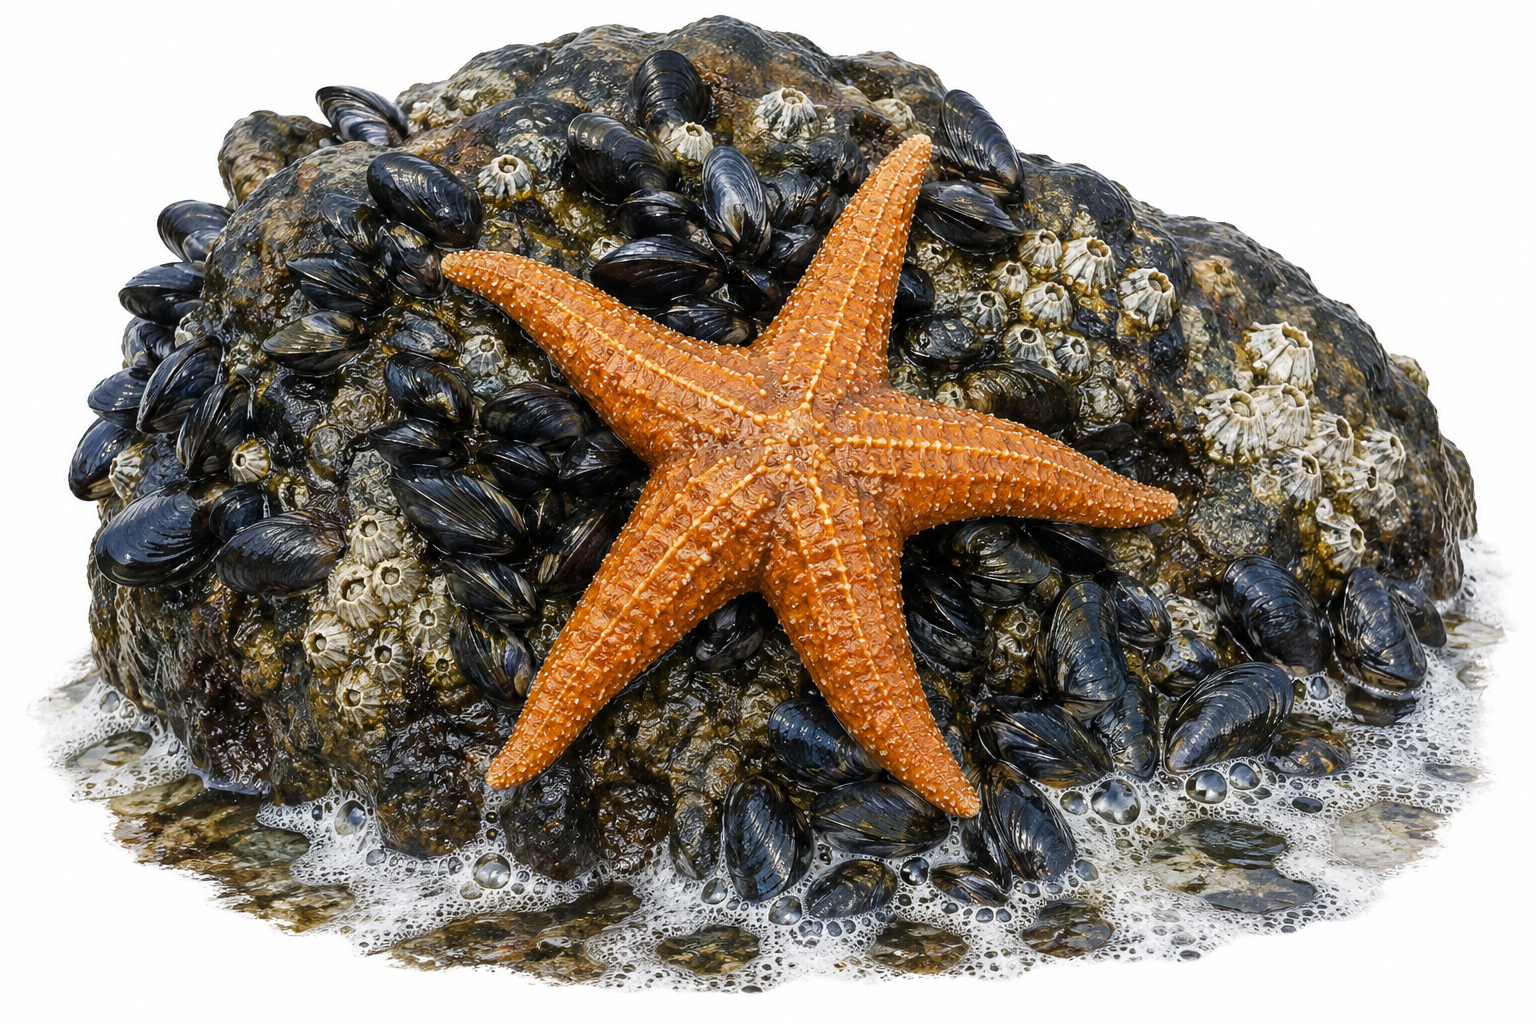
\includegraphics[width=0.6\linewidth]{images/book3/ai/b3-27-sea-star-mussels.png}

{\small Una estrella de mar depredadora sobre un banco de mejillones en
marea baja: el depredador clave cuya retirada convirtió una costa de quince
especies en un monocultivo de mejillones.}
\end{omfigure}

\section{Vivir juntos: parasitismo, mutualismo, comensalismo}

\begin{definition}[Parasitismo, simbiosis, mutualismo]\label{def:b1:species-interactions:symbiosis}
\index{simbiosis}\index{parásito}\index{liquen}
Un \emph{parásito} vive a expensas de un hospedador, sobre él (ectoparásito:
garrapata, piojo, muérdago) o dentro de él (endoparásito: tenia, parásito
del paludismo, hongo de la roya), y le toma nutrientes y le reduce la
eficacia biológica sin matarlo necesariamente; los parásitos suelen estar
especializados, con ciclos vitales complejos a través de varios
hospedadores. Una \emph{simbiosis} es cualquier asociación estrecha y
duradera entre dos especies; un \emph{\omterm{def:b1:species-interactions:types}{mutualismo}} es la que beneficia a
ambas: la \omterm{def:b1:plant-water-minerals:mycorrhiza}{micorriza} (un hongo sobre las raíces de una planta, o dentro de
ellas, que cambia fosfato y agua por azúcar;
\cref{ch:b1:plant-water-minerals}), el \omterm{def:b1:plant-water-minerals:nodules}{nódulo radicular} (bacterias fijadoras
de nitrógeno alimentadas por la leguminosa), el \emph{liquen} (un hongo que
aloja un alga o una cianobacteria), el coral de arrecife (un cnidario que
aloja dinoflagelados fotosintéticos), la microbiota intestinal de un
rumiante o de una termita (\cref{ch:b1:digestion-absorption}) y la
polinización (néctar a cambio de transporte de polen). Muchos \omterm{def:b1:species-interactions:types}{mutualismos}
empezaron como \omterm{def:b1:species-interactions:types}{parasitismos} o depredaciones que la coevolución de los socios
volvió de provecho mutuo, y siguen siendo condicionales: un hongo
micorrícico en un suelo rico en fosfato es un coste, y la planta lo reduce.
\end{definition}

\begin{example}[La polinización como intercambio]\label{ex:b1:species-interactions:pollination}
Una flor gasta unos pocos julios de azúcar en néctar; una abeja gasta vuelo
en recogerlo y lleva polen de flor en flor por el camino. El color, el
aroma, la forma y el calendario de la flor van dirigidos a sus
polinizadores, y la longitud de la lengua de la abeja, su visión en color y
su memoria de forrajeo, a sus flores; algunas parejas encajan tan
estrechamente --- un largo espolón de néctar y la única polilla cuya lengua
lo alcanza --- que ninguno sobrevive sin el otro, y toda una \omterm{def:b1:ecosystem-organization:ecosystem}{comunidad}
vegetal puede depender de unas pocas especies de insecto.
\end{example}

\begin{omfigure}
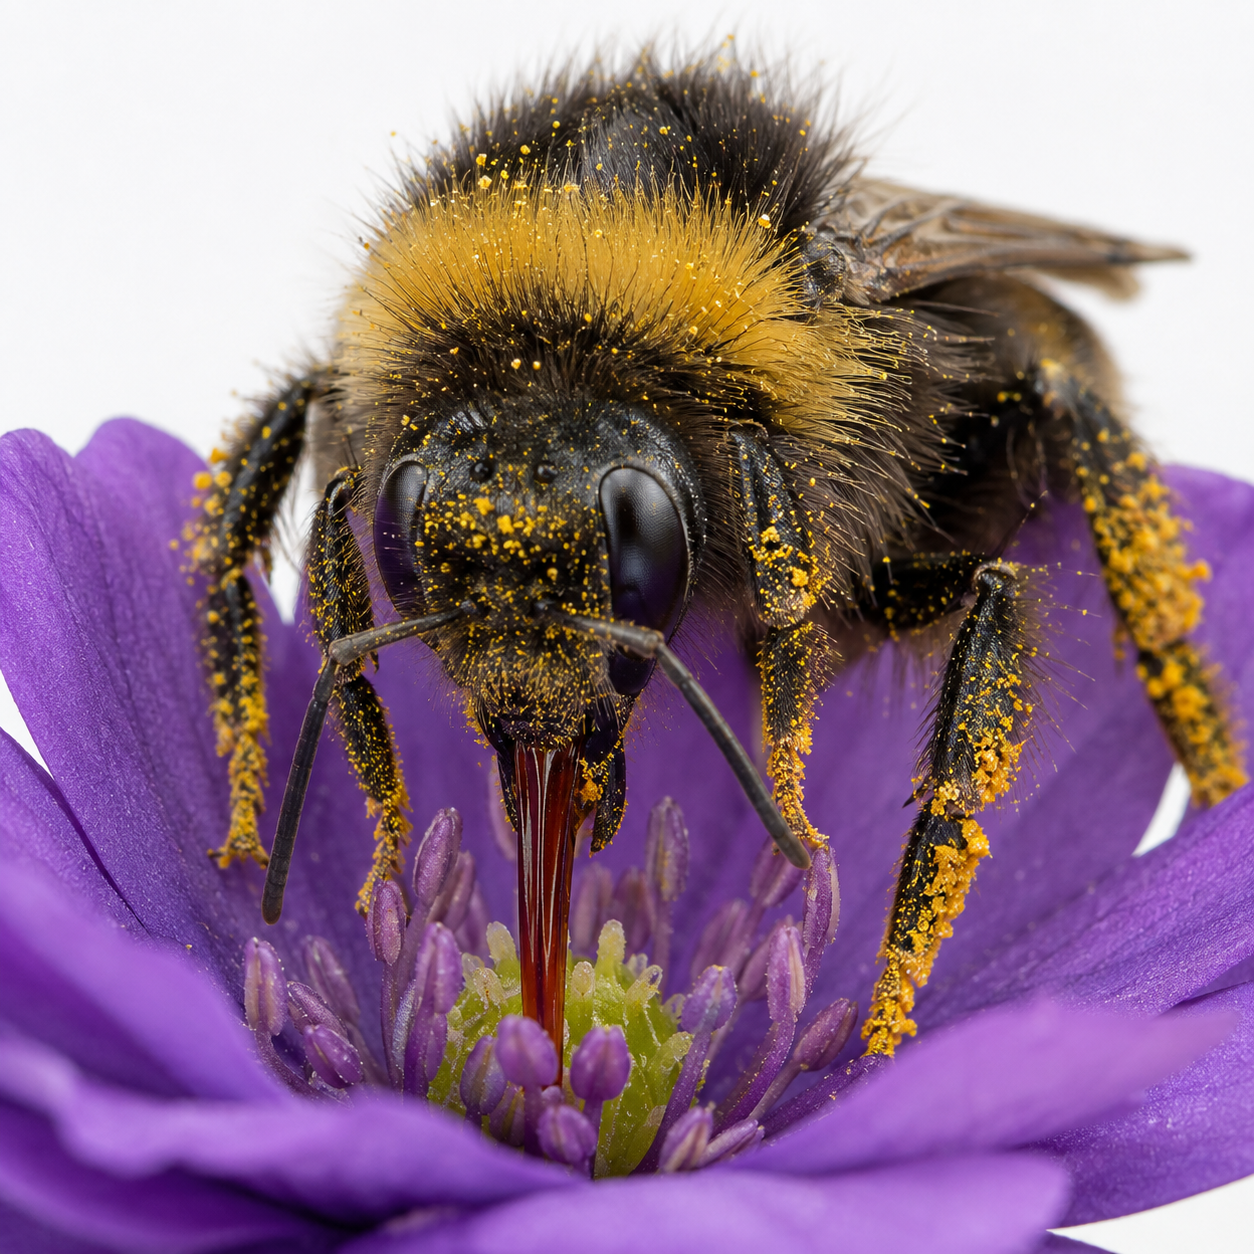
\includegraphics[width=0.56\linewidth]{images/book3/ai/b3-27-bee-flower.png}

{\small Un \omterm{def:b1:species-interactions:types}{mutualismo} en acción: néctar para la abeja, transporte de polen
para la flor. La forma de cada socio la ha modelado el otro.}
\end{omfigure}

\begin{remark}[El comensalismo es raro e inestable]\label{rem:b1:species-interactions:commensal}
Pocas interacciones son verdaderamente $+/0$: la epífita que da sombra a su
hospedador, la rémora que le cuesta a su tiburón un poco de resistencia al
avance, la garcilla bueyera que come lo que el ganado levanta son comensales
solo hasta donde llega la precisión de la medida. Las interacciones se
clasifican por su efecto neto, y el efecto neto puede cambiar con las
condiciones.
\end{remark}

\section{Interacciones que modelan la comunidad}

\begin{definition}[Especie clave, cascada trófica]\label{def:b1:species-interactions:keystone}
\index{especie clave}\index{cascada trófica}
Una \emph{especie clave} es aquella cuyo efecto sobre la \omterm{def:b1:ecosystem-organization:ecosystem}{comunidad} es
desproporcionado respecto de su abundancia o su biomasa: retírese y la
estructura de la \omterm{def:b1:ecosystem-organization:ecosystem}{comunidad} cambia, por lo general porque controlaba a un
competidor dominante. Una \emph{cascada trófica} es la propagación de un
efecto por una \omterm{def:b1:ecosystem-organization:foodweb}{cadena alimentaria} a través de más de un nivel: la presencia
de un depredador rebaja los herbívoros, lo que eleva las plantas; su
retirada hace lo contrario. Las cascadas muestran que las \omterm{def:b1:ecosystem-organization:ecosystem}{comunidades} se
estructuran tanto desde arriba como desde abajo (por la productividad,
\cref{ch:b1:ecosystem-organization}).
\end{definition}

\begin{proposition}[Un depredador puede mantener la diversidad]\label{prop:b1:species-interactions:paine}
Al comerse a la especie que de otro modo ganaría la \omterm{def:b1:species-interactions:types}{competencia} por el
espacio o por los recursos, un depredador mantiene en la \omterm{def:b1:ecosystem-organization:ecosystem}{comunidad} a las
perdedoras; su retirada permite al competidor dominante excluirlas, y la
diversidad cae.
\end{proposition}
\begin{proof}[Evidencia]
Paine (1966) retiró la estrella de mar \emph{Pisaster} de un tramo de
\qty{8}{m} de costa rocosa del Pacífico de América del Norte y dejó un tramo
vecino como control. La estrella de mar come mejillones, percebes y otros
animales sésiles, y prefiere los mejillones. En dos años el mejillón
\emph{Mytilus} se había extendido roca abajo y había ocupado casi todo el
espacio; los percebes, quitones, lapas y algas que habían vivido en los
huecos desaparecieron, y las quince especies de la parcela control cayeron a
ocho. La parte de la biomasa de la \omterm{def:b1:ecosystem-organization:ecosystem}{comunidad} que correspondía al propio
depredador era pequeña; su retirada lo cambió todo.
\end{proof}

\begin{omfigure}
\begin{tikzpicture}
\begin{axis}[
  width=0.74\linewidth, height=5.6cm,
  axis x line=bottom, axis y line=left,
  xmin=1963, xmax=1969, ymin=0, ymax=18,
  xlabel={año}, ylabel={especies en la parcela},
  xlabel style={font=\small}, ylabel style={font=\small},
  tick label style={font=\small}, xtick={1963,1964,1965,1966,1967,1968},
  x tick label style={/pgf/number format/1000 sep=},
  legend style={font=\scriptsize, at={(0.98,0.03)}, anchor=south east, draw=none, fill=none},
  legend cell align=left,
]
\addplot[omDef, very thick, mark=*] coordinates {(1963,15) (1964,15) (1965,14) (1966,15) (1967,15) (1968,15)};
\addlegendentry{control: estrella de mar presente}
\addplot[omThm, very thick, mark=square*] coordinates {(1963,15) (1964,12) (1965,10) (1966,9) (1967,8) (1968,8)};
\addlegendentry{estrella de mar retirada}
\node[font=\scriptsize, anchor=south west, align=left] at (axis cs:1966.2,10.6) {los mejillones\\ toman la roca};
\end{axis}
\end{tikzpicture}

{\small El experimento de retirada de Paine (a partir de sus datos). La
diversidad de la parcela sin el depredador cae a la mitad en cinco años,
mientras que el control conserva sus quince especies.}
\end{omfigure}

\begin{example}[Lobos, uapitíes y sauces]\label{ex:b1:species-interactions:wolves}
Los lobos fueron exterminados de un gran parque de montaña en la década de
1920; sus uapitíes se multiplicaron y ramonearon hasta dejar en tocones los
sauces y los álamos temblones de las orillas; los castores, que necesitan
sauce, menguaron; las aves cantoras perdieron sus matorrales. Cuando los
lobos se reintrodujeron en 1995, los uapitíes decayeron y, lo que importa
más, evitaron los fondos de valle donde eran vulnerables; los sauces
rebrotaron, los castores volvieron y construyeron presas, y los humedales
que crearon trajeron de vuelta peces, anfibios y aves. La cascada corrió
desde un carnívoro por un herbívoro hasta las plantas y desde ahí hasta una
docena de especies que nunca se cruzaron con un lobo --- con el tiempo, la
caza y otros depredadores aportando lo suyo, de modo que la parte que
corresponde a los lobos sigue debatiéndose.
\end{example}

\begin{omfigure}
\begin{tikzpicture}[font=\footnotesize, >=Stealth, line cap=round,
  lv/.style={draw, thick, rounded corners=3pt, inner sep=4pt, align=center, fill=white, minimum width=2.6cm}]
  \node[lv, fill=omDef!25] (wolf) at (0,4.5) {lobos};
  \node[lv, fill=omProp!20] (elk) at (0,2.8) {uapitíes};
  \node[lv, fill=omExo!20] (willow) at (0,1.1) {sauces, álamos};
  \node[lv, fill=omProp!20] (beaver) at (3.8,1.1) {castores};
  \node[lv, fill=omDef!12] (wet) at (7.4,1.1) {charcas, humedales};
  \node[lv, fill=omThm!15] (birds) at (3.8,-0.6) {aves cantoras, peces,\\ anfibios};
  \draw[->, very thick, omThm] (wolf) -- (elk) node[midway, right] {$-$: menos, y apartados de las orillas};
  \draw[->, very thick, omThm] (elk) -- (willow) node[midway, left] {$-$: ramoneo};
  \draw[->, very thick, omDef] (willow) -- (beaver) node[midway, above=9pt] {$+$: alimento, presas};
  \draw[->, very thick, omDef] (beaver) -- (wet) node[midway, above] {$+$};
  \draw[->, very thick, omDef] (willow) -- (birds) node[midway, below left] {$+$};
  \draw[->, very thick, omDef] (wet) |- (birds) node[pos=0.8, below] {$+$};
  \node[anchor=north, align=center, gray] at (3.4,-1.5) {dos signos menos dan un más: el regreso de los lobos aumentó los sauces,\\ y los sauces llevaron el efecto a especies que los lobos nunca tocaron};
\end{tikzpicture}

{\small Una \omterm{def:b1:species-interactions:keystone}{cascada trófica}: un efecto que baja tres niveles y se propaga
de lado por la \omterm{def:b1:ecosystem-organization:ecosystem}{comunidad}. Los signos dan el sentido de cada eslabón.}
\end{omfigure}

\begin{omfigure}
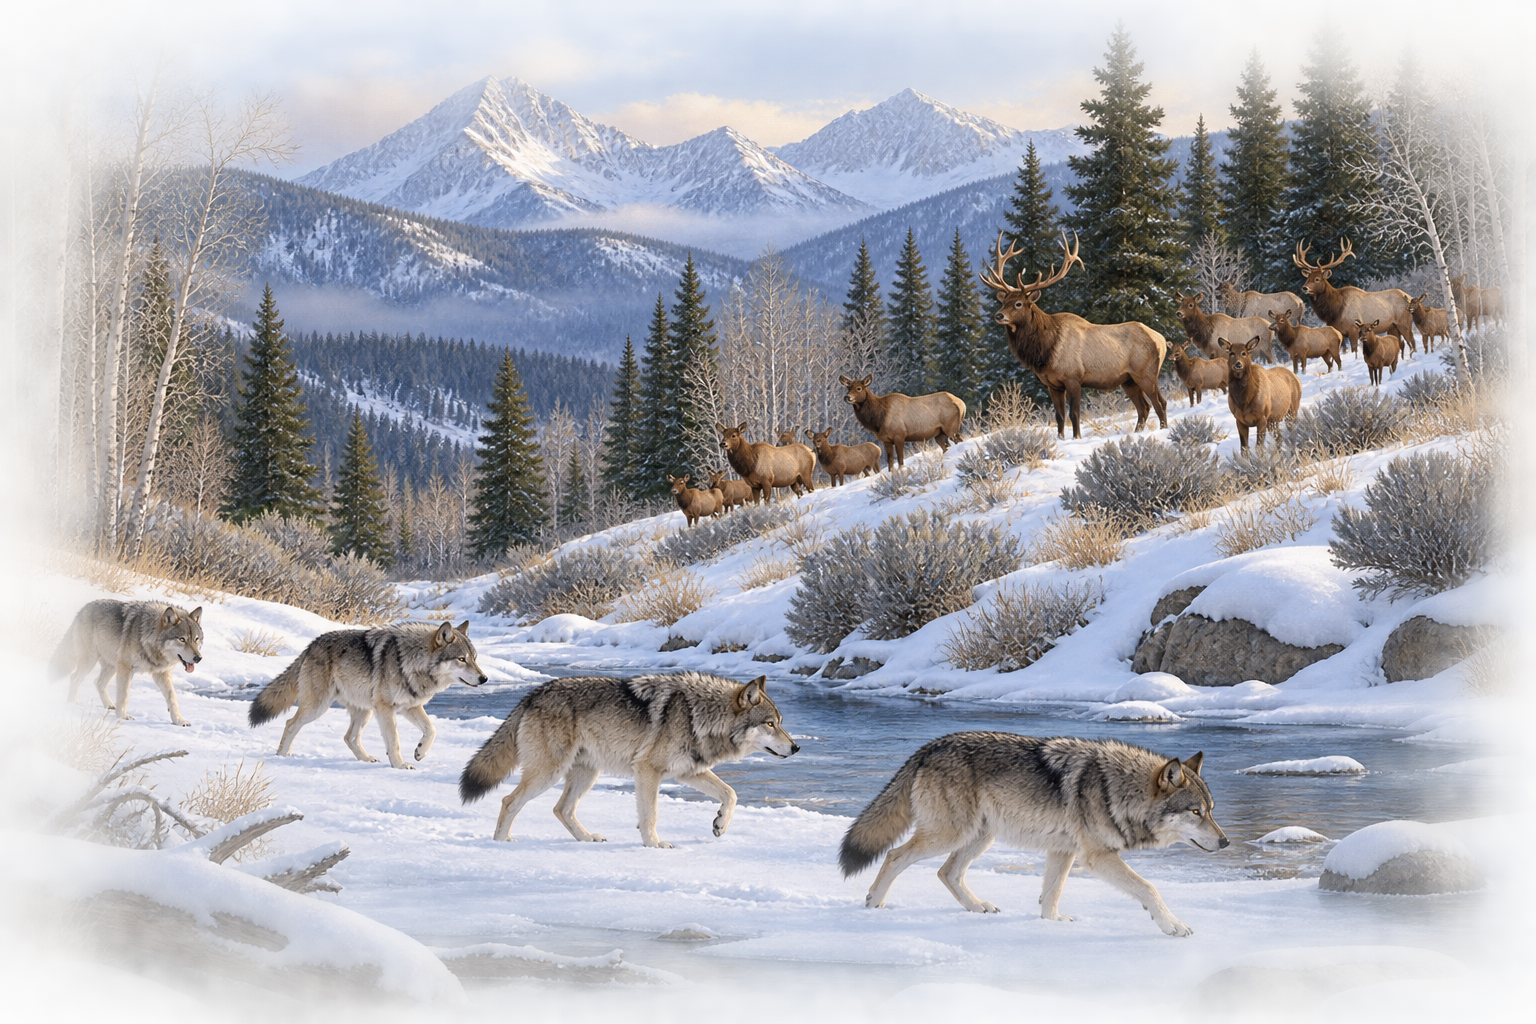
\includegraphics[width=0.6\linewidth]{images/book3/ai/b3-27-wolves-elk.png}

{\small Lobos y uapitíes en un valle fluvial en invierno. El efecto del
depredador sobre la vegetación pasa tanto por dónde se atreven a pastar los
uapitíes como por cuántos son.}
\end{omfigure}

\begin{method}[Lectura de una interacción a partir de un experimento]\label{met:b1:species-interactions:reading}
\begin{enumerate}
  \item Identifíquense la manipulación (retirada, adición, jaula de
        exclusión, emparejamiento en cultivo) y el control mantenido junto a
        ella en las mismas condiciones.
  \item Para cada especie, compárese su abundancia con y sin el socio: el
        signo de la diferencia da el signo de la interacción sobre esa
        especie.
  \item Búsquense los efectos indirectos: una especie que cambió sin tocar a
        la manipulada está al final de una cadena --- encuéntrense los
        intermediarios.
  \item Compruébense la escala temporal (una \omterm{def:b1:species-interactions:types}{competencia} puede tardar muchas
        generaciones en resolverse; una cascada corre al ritmo del nivel más
        lento) y la escala espacial (¿se sostiene el resultado más allá de
        la parcela?).
  \item Ajústese el modelo donde los datos lo permitan: curvas logísticas e
        \omterm{prop:b1:species-interactions:lotka}{isoclinas} para la \omterm{def:b1:species-interactions:types}{competencia}, la \omterm{thm:b1:species-interactions:holling}{ecuación del disco} para una
        \omterm{def:b1:species-interactions:functional}{respuesta funcional}, y léanse los parámetros en las
        representaciones linealizadas.
\end{enumerate}
\end{method}

\section{Ejercicios}

\begin{exercise}[$\star$]\label{exo:b1:species-interactions:1}
Dese el par de signos y un ejemplo de cada uno de los seis tipos de
interacción.
\end{exercise}

\begin{exercise}[$\star$]\label{exo:b1:species-interactions:2}
Enúnciese el principio de \omterm{def:b1:species-interactions:competition}{exclusión competitiva} y dígase por qué no prohíbe
cinco reinitas en una misma picea.
\end{exercise}

\begin{exercise}[$\star$]\label{exo:b1:species-interactions:3}
Defínanse \omterm{def:b1:species-interactions:functional}{tiempo de manipulación} y tasa de ataque, y dese la tasa máxima de
alimentación de un depredador con $h = \qty{30}{min}$.
\end{exercise}

\begin{exercise}[$\star$]\label{exo:b1:species-interactions:4}
¿Qué es una \omterm{def:b1:species-interactions:keystone}{especie clave}? ¿Por qué una \omterm{def:b1:species-interactions:keystone}{especie clave} no es simplemente la
más abundante?
\end{exercise}

\begin{exercise}[$\star\star$]\label{exo:b1:species-interactions:5}
La especie 1 tiene $K_1 = 500$ y la especie 2, $K_2 = 400$, con $\alpha =
0.5$ y $\beta = 0.6$. Dibújense las \omterm{prop:b1:species-interactions:lotka}{isoclinas} y dese el desenlace. Repítase
con $\alpha = 2$, $\beta = 0.6$.
\end{exercise}

\begin{exercise}[$\star\star$]\label{exo:b1:species-interactions:6}
Un depredador con $a = \qty{0.2}{m^2/h}$ y $h = \qty{0.25}{h}$ encuentra
presas a \qty{10}{} y a \qty{100}{} por metro cuadrado. Calcúlense su tasa
de alimentación en cada caso y la densidad a la que está semisaturado.
\end{exercise}

\begin{exercise}[$\star\star$]\label{exo:b1:species-interactions:7}
¿Por qué una respuesta de tipo III estabiliza una \omterm{def:b1:populations:population}{población} de presas a baja
densidad y una de tipo II no?
\end{exercise}

\begin{exercise}[$\star\star$]\label{exo:b1:species-interactions:8}
A partir del experimento de Gause, explíquese por qué \emph{P.~bursaria}
coexistió con \emph{P.~aurelia} y \emph{P.~caudatum} no. ¿Qué marcó la
diferencia: la tasa de crecimiento o el \omterm{def:b1:ecosystem-organization:niche}{nicho}?
\end{exercise}

\begin{exercise}[$\star\star$]\label{exo:b1:species-interactions:9}
Un mimético batesiano se vuelve más común que su modelo tóxico. Predígase
qué le ocurre a la protección de ambos, y por qué el éxito del mimético se
limita a sí mismo.
\end{exercise}

\begin{exercise}[$\star\star\star$]\label{exo:b1:species-interactions:10}
La parcela de retirada de Paine perdió siete especies. Explíquese, con el
modelo de las \omterm{prop:b1:species-interactions:lotka}{isoclinas}, cómo un depredador que se come al competidor
dominante convierte una exclusión en una coexistencia.
\end{exercise}

\begin{exercise}[$\star\star\star$]\label{exo:b1:species-interactions:11}
Un hongo micorrícico se lleva el \qty{15}{\%} del fotosintato de una planta
y le suministra el \qty{80}{\%} de su fosfato. ¿En qué condiciones es la
asociación un \omterm{def:b1:species-interactions:types}{mutualismo}, y en cuáles un \omterm{def:b1:species-interactions:types}{parasitismo}? Propóngase un
experimento para distinguirlo.
\end{exercise}

\begin{exercise}[$\star\star\star$]\label{exo:b1:species-interactions:12}
Diséñese un experimento para comprobar si fueron los lobos, y no el tiempo o
la caza, los que causaron la recuperación de los sauces: controles,
réplicas, las variables que medir y qué resultado refutaría la cascada.
\end{exercise}

\section{Problema: el depredador y la costa}

\begin{problem}[{Problema de fin de semana --- los ciliados de Gause en un
tubo, los datos de alimentación de un depredador ajustados a la ecuación del
disco, la costa de Paine con y sin su estrella de mar, y el balance de un
polinizador, hasta llegar a la tasa de ataque y al tiempo de manipulación
del depredador}]
\label{pb:b1:species-interactions:1}

\medskip
\noindent\textbf{Parte I --- \omterm{def:b1:species-interactions:types}{Competencia} en un tubo.}
Se cultivan dos ciliados por separado: la especie A alcanza $K_A = 200$ por
\qty{0.5}{mL} con $r_A = \qty{0.8}{d^{-1}}$; la especie B alcanza
$K_B = 130$ con $r_B = \qty{0.55}{d^{-1}}$. Juntas, un individuo de B
consume tanto alimento como $\alpha = 1.4$ de A, y un individuo de A tanto
como $\beta = 0.9$ de B.
\begin{enumerate}
  \item Escríbanse las dos \omterm{prop:b1:species-interactions:lotka}{isoclinas} y sus cortes con los ejes.
  \item Dibújense y dígase qué especie gana, y por qué el desenlace no
        depende de los efectivos de partida.
  \item A partir de los tiempos de duplicación ($\ln 2/r$), ¿qué especie
        habría cabido esperar que ganara solo por la tasa de crecimiento?
  \item Una tercera especie C se alimenta en el fondo del tubo y compite con
        A solo débilmente ($\alpha = 0.3$, $\beta = 0.3$, $K_C = 100$).
        Dibújense las \omterm{prop:b1:species-interactions:lotka}{isoclinas} y dese el desenlace.
  \item ¿Por qué se cumple el principio de exclusión en un tubo y falla tan
        a menudo en un bosque? Dense dos razones.
  \item Calcúlense los efectivos de equilibrio de A y de C a partir del
        cruce de las \omterm{prop:b1:species-interactions:lotka}{isoclinas}.
\end{enumerate}

\medskip
\noindent\textbf{Parte II --- La \omterm{thm:b1:species-interactions:holling}{ecuación del disco}.}
Se ofrecen a un escarabajo depredador presas a densidades de 5, 10, 20, 40 y
80 por metro cuadrado; come respectivamente 2,0, 3,3, 5,0, 6,7 y 8,0 presas
al día.
\begin{enumerate}[resume]
  \item Represéntese la tasa de alimentación frente a la densidad e
        identifíquese el tipo de respuesta.
  \item Calcúlense $1/f$ y $1/N$ para cada punto y represéntense.
  \item A partir de la pendiente y de la ordenada en el origen, obténganse
        $a$ y $h$.
  \item Calcúlense la tasa máxima de alimentación y la densidad de
        semisaturación.
  \item ¿En cuál de las cinco densidades dedica el escarabajo más de la
        mitad de su tiempo a manipular?
  \item Las presas del escarabajo crecen logísticamente con
        $r = \qty{0.1}{d^{-1}}$ y $K = 200$. ¿A qué densidad iguala el
        crecimiento de las presas (por metro cuadrado sin escarabajos) al
        consumo del escarabajo si hay un escarabajo por metro cuadrado? ¿Es
        estable ese equilibrio frente a una pequeña subida de las presas?
  \item Aparece una segunda especie de presa que el escarabajo manipula al
        doble de velocidad. Predígase el cambio de la ingesta total del
        escarabajo a densidad alta.
\end{enumerate}

\medskip
\noindent\textbf{Parte III --- La costa.}
En la parcela control de Paine la \omterm{def:b1:ecosystem-organization:ecosystem}{comunidad} tenía 15 especies; en la parcela
de retirada el recuento cayó 15, 12, 10, 9, 8, 8 a lo largo de cinco años, y
la cobertura de mejillones sobre la roca subió del \qty{20}{\%} al \qty{85}{\%}.
\begin{enumerate}[resume]
  \item Calcúlese el \omterm{def:b1:ecosystem-organization:diversity}{índice de Shannon} de una parcela con 15 especies con
        igual abundancia, y el de una con 8 especies donde los mejillones
        son el \qty{85}{\%} de los individuos y las otras siete se reparten
        el resto por igual.
  \item ¿En qué factor cayó la diversidad?
  \item Explíquese, con los signos de las interacciones, por qué retirar una
        interacción $+/-$ (la \omterm{def:b1:species-interactions:types}{depredación} sobre los mejillones) reforzó una
        $-/-$ (la \omterm{def:b1:species-interactions:types}{competencia} por la roca).
  \item La estrella de mar era menos del \qty{1}{\%} de la biomasa de la
        parcela. ¿Por qué es la biomasa una mala guía de la importancia de
        una especie?
  \item Predígase qué habría ocurrido si la presa preferida de la estrella
        de mar hubiera sido la especie más rara y no la dominante.
  \item Propóngase una manera de confirmar que fue la \omterm{def:b1:species-interactions:types}{depredación} sobre los
        mejillones y no algún otro efecto de la estrella de mar (un
        experimento de jaulas).
\end{enumerate}

\medskip
\noindent\textbf{Parte IV --- El balance de un \omterm{def:b1:species-interactions:types}{mutualismo}.}
Una abeja visita 1000 flores en un día y recoge \qty{40}{mg} de azúcar; cada
flor da \qty{40}{\micro g} de azúcar en néctar y recibe polen de, en
promedio, 3 flores anteriores por visita. La planta gasta el \qty{1}{\%} de
su fotosintato diario (\qty{4}{mg} de azúcar por flor) en néctar; el vuelo
de una abeja cuesta \qty{0.5}{mg} de azúcar por hora de forrajeo
(\qty{8}{h}).
\begin{enumerate}[resume]
  \item Calcúlense la ganancia neta diaria de azúcar de la abeja y su
        equivalente energético a \qty{16}{kJ/g}.
  \item Calcúlese el coste diario de la planta por flor como fracción de su
        fotosintato y dígase qué compra con él.
  \item ¿Por qué es esta interacción $+/+$ aunque cada socio esté explotando
        al otro?
  \item Un ladrón de néctar muerde la base de la flor y se lleva el néctar
        sin tocar el polen. Dense los signos de la interacción
        ladrón--planta y su efecto probable sobre la abeja.
  \item Dibújese el diagrama de signos de la planta, la abeja, el ladrón y
        un ave que come ladrones, y predígase el efecto indirecto del ave
        sobre la planta.
  \item Enúnciese el resultado: la tasa de ataque y el \omterm{def:b1:species-interactions:functional}{tiempo de
        manipulación} del escarabajo, y su tasa máxima de alimentación.
\end{enumerate}
\end{problem}
